\lstdefinelanguage{plaintext}{
  sensitive=false,
  comment=[l]{//},
  morecomment=[s]{/*}{*/},
  identifierstyle=\color{black},
  morestring=[b]',
  morestring=[b]"
}

\lstset
{ 
    language=plaintext,
    basicstyle=\footnotesize,
    numbers=left,
    stepnumber=1,
    showstringspaces=false,
    tabsize=1,
    breaklines=true,
    breakatwhitespace=false,
    frame=leftline
}

\chapter{Implementasi dan Pengujian}
\label{chap:implementasiDanPengujian}

Pada bab ini dibahas mengenai implementasi perangkat lunak dan pengujian yang dilakukan terhadap perangkat lunak tersebut. Lingkungan implementasi, yang meliputi perangkat keras dan perangkat lunak, serta hasil implementasi akan dijelaskan pada bab ini. Selain Pengujian yang dilakukan pada skripsi ini, yang meliputi pengujian fungsional dan eksperimental akan dijelaskan pada bab ini.

\section{Implementasi}
Pada bagian ini akan dijelaskan mengenai lingkungan yang digunakan untuk membangun perangkat lunak beserta hasil implementasinya.

\subsection{Lingkungan Implementasi}
Berikut spesifikasi perangkat keras dan perangkat lunak yang digunakan dalam pembangunan pada skripsi ini:

\begin{enumerate}
	\item Spesifikasi Perangkat Keras
	
		\begin{itemize}
			\item Perangkat: Laptop
			\item Processor: AMD Bristol Ridge Quad Core FX-9830P 3GHz
			\item RAM: 8GB
			\item GPU: Radeon RX 460
			\item Storage: Harddisk 1TB
		\end{itemize}		

	\item Spesifikasi Perangkat Lunak

		\begin{itemize}
			\item Sistem Operasi Windows 10 64-bit
			\item PHP 7.3.5 (cli)
			\item Composer versi 1.8.5
			\item Sublime Text versi 3.2.1
		\end{itemize}	
	
\end{enumerate}

\subsection{Hasil Implementasi}
Perangkat lunak dibangun menggunakan bahasa pemrograman \textit{PHP} dan \textit{library PdfParser}. Perangkat lunak tidak memiliki \textit{Graphical User Interface}, sehingga seluruh kegiatan dilakukan melalui terminal. Perangkat lunak akan menerima input berupa file PDF skripsi yang disimpan pada folder yang telah disediakan, dan mengeluarkan laporan kesalahan pada terminal.

\begin{lstlisting}[caption={Perintah yang digunakan untuk menjalankan perangkat lunak}	\label{lst:command},language=php,xleftmargin=.3\textwidth] 
php main.php ../res/nama_file.pdf
\end{lstlisting}
\medskip

Listing \ref{lst:command} merupakan perintah yang perlu dituliskan pada terminal, untuk menjalankan perangkat lunak. Kelas Main menjadi kelas yang digunakan untuk menjalankan seluruh proses yang berjalan dalam perangkat lunak. File PDF skripsi yang akan diperiksa harus berada di folder yang telah disediakan, yaitu pada folder Skripsi$\backslash$src$\backslash$res. Nama file yang digunakan pada umumnya sesuai dengan \textit{template} skripsi yang diberikan, yaitu ''skripsi.pdf''. Namun pengguna juga dapat menggunakan nama yang berbeda, yang paling utama file tersebut memiliki ekstensi PDF.

\begin{figure}[H]
	\centering	
	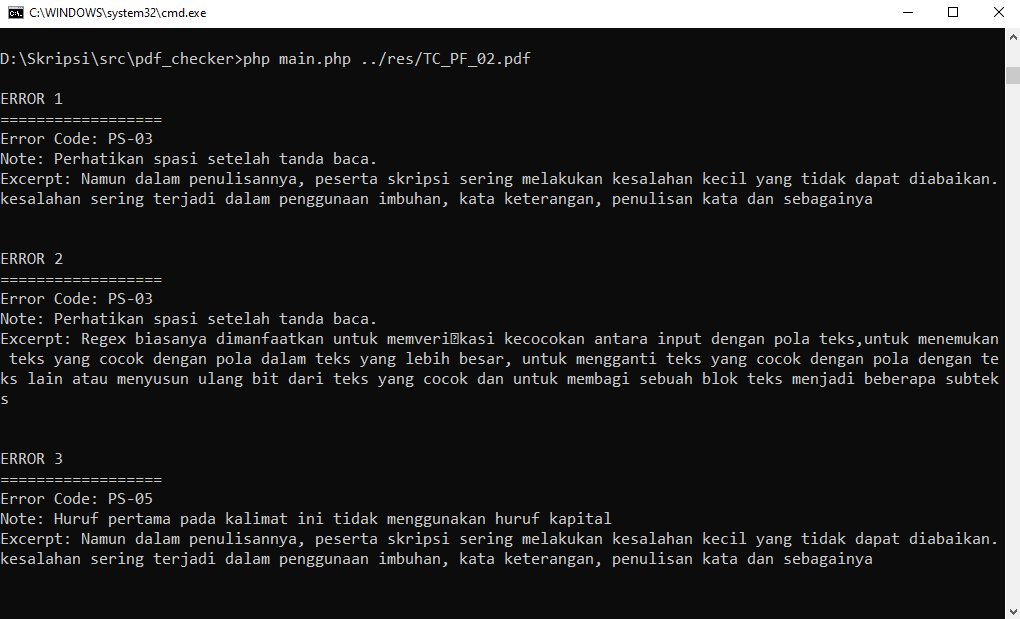
\includegraphics[scale=0.65]{hasil-implementasi.png}
	\caption{Laporan Kesalahan}	
	\label{fig:error_report} 
\end{figure}
\medskip

Gambar \ref{fig:error_report} merupakan hasil laporan yang dikeluarkan oleh perangkat lunak melalui \textit{terminal windows}. Informasi yang diberikan oleh laporan tersebut yaitu, kode kesalahan, jenis kesalahan yang ditemukan dan kesalahan yang ditemukan. Laporan kesalahan yang dikeluarkan sudah diurutkan dari fitur pertama hingga terakhir, yaitu dari fitur PS-01 hingga NAT-03.

\section{Pengujian}
Pada bagian ini akan dijelaskan mengenai pengujian yang dilakukan pada perangkat lunak. Akan dilakukan 2 bentuk pengujian pada skripsi ini, yaitu pengujian fungsional dan pengujian eksperimental.

\subsection{Pengujian Fungsional}
Pengujian fungsional bertujuan untuk menguji fungsionalitas perangkat lunak. Perangkat lunak memiliki 8 fitur yang telah diimplementasikan. Fitur-fitur tersebut akan diuji untuk melihat kebenaran dan kesesuaian fitur tersebut dengan yang diharapkan. Pada pengujian ini, perangkat lunak akan diuji dengan 2 buah \textit{test case} dokumen skripsi Informatika Unpar dengan mode sidang akhir. Kedua \textit{test case} yang digunakan yaitu, ''TC\_PF\_01.pdf'' dan ''TC\_PF\_02.pdf''. Isi dari ke-2 file tersebut sama, namun pada file ''TC\_PF\_02.pdf'' sudah disisipkan kesalahan-kesalahan yang dapat dideteksi oleh setiap fitur yang ada. Berikut ini adalah rincian dari kesalahan-kesalahan yang dimasukan ke dalam \textit{test case} tersebut.

\begin{enumerate}
	\item Pada halaman cover bahasa Indonesia dan bahasa Inggris, data yang meliputi judul, nama mahasiswa, npm mahasiswa, dan yang lainnya tidak diisi. Hal ini dilakukan untuk menguji fitur pemeriksa kelengkapan data skripsi (KAL-03).
	
	\item Pada bab 1, hampir seluruh karakter pertama dalam kalimat menggunakan huruf kecil. Hal ini dilakukan untuk menguji fitur pemeriksa huruf kapital (PS-05).
	
	\item Pada bab 2, terdapat 2 buah teori yang referensinya tidak dirujuk dengan baik. Hal ini dilakukan untuk menguji fitur pemeriksa referensi (NAT-01).
	
	\item Pada bab 3, terdapat beberapa kata yang diketik tidak sesuai dengan kamus. Hal ini dilakukan untuk menguji fitur pemeriksa kata (PS-01). Selain itu pada bab ini tidak diberikan kata pengantar sebelum memulai subbab, untuk menguji fitur pemeriksa kata pengantar pada bab (KAL-02).
	
	\item Pada bab 4, terdapat beberapa kata yang tidak diberikan karakter spasi sebelum ataupun setelah tanda baca. Hal ini dilakukan untuk menguji fitur pemeriksa karakter spasi sebelumm atau setelah tanda baca (PS-03).	

		\item Pada bab 5, hanya terdapat 1 sub sub bab dalam sebuah sub bab. Hal ini dilakukan untuk menguji fitur pemeriksa jumlah subbab (PS-09).	
		
	\item Untuk menguji fitur pemeriksa kata ganti orang (VAN-03), pada setiap bab disisipkan kata ganti orang.
\end{enumerate}

\textit{Test case} yang dipakai menggunakan template dokumen skripsi . Hasil dari pengujian tersebut akan dijelaskan pada tabel \ref{tab:pengujian_fungsional}.

\begin{table}[H]
	\renewcommand{\arraystretch}{1.5}
	\caption {Tabel Pengujian Fungsional} 	
	\label{tab:pengujian_fungsional}
	\begin{center}
		\begin{tabular}{|p{2.5 cm}|>{\raggedright} p{6.0 cm}| p{6.0 cm}|}
		\hline
		Kasus Uji & Hasil yang diharapkan & Hasil pengujian \\ 
		\hline
		Fitur PS-01 & Program berhasil menemukan kata-kata yang tidak terdapat pada kamus & Sesuai \\ 
		\hline
		Fitur PS-03 & Program berhasil kata-kata yang tidak diberi spasi setelah tanda baca & Sesuai \\ 
		\hline 
		Fitur PS-05 & Program berhasil menemukan karakter pertama pada kalimat yang tidak menggunakan huruf kapital & Sesuai \\ 
		\hline 
		Fitur PS-09 & Program berhasil menemukan bab yang hanya memiliki satu subbab & Sesuai \\ 
		\hline
		Fitur KAL-02 & Program berhasil menemukan bab atau subbab yang tidak diberi kata pengantar & Sesuai \\
		\hline
		Fitur KAL-03 & Program berhasil menemukan data skripsi yang belum diisi  & Sesuai \\
		\hline
		Fitur NAT-01 & Program berhasil menemukan referensi yang tidak dirujuk dengan baik & Sesuai \\
		\hline
		Fitur VAN-03 & Program berhasil menemukan kata ganti orang pada kalimat & Sesuai \\ 
		\hline
		\end{tabular}
	\end{center}
\end{table}

\subsection{Pengujian Eksperimental}
Pada pengujian eksperimental, perangkat lunak akan diuji dengan 5 buah \textit{test case} dokumen skripsi yang diambil dari \textit{Github} skripsi Informatika.

\begin{itemize}
	\item TC\_PE\_01.pdf~\cite{pe01}
	\item TC\_PE\_02.pdf~\cite{pe02}
	\item TC\_PE\_03.pdf~\cite{pe03}
	\item TC\_PE\_04.pdf~\cite{pe04}
	\item TC\_PE\_05.pdf~\cite{pe05}
\end{itemize}
